\section{Auswertung}
\subsection{Messung des Erdmagnetfeldes}
Wie in der Durchführung bereits beschrieben, musste die horizontale Komponente
des Erdmagnetfeldes kompensiert werden. Während der Messung wurde die Stärke des
gesamten Horizontalfeldes (Sweepfeld + Horizontal) in Abhängigkeit von der Resonanzfrequenz von beiden
Isotope gemessen. Zu diesem Zweck wurde der Strom erhöht, bis die jeweiligen
Resonanzstellen zu sehen waren. Mit der Helmholtz-Gleichung
\begin{equation}
  B = \symup{\mu_0} \, \frac{8 \, I \, N}{\sqrt{125}\, R} \, ,
  \label{eqn:helmholtz}
\end{equation}
wobei $I$ der Strom, $N$ die Windungszahl der Helmholtzspule und $R$ der Spulenradius
ist, werden die Magnetfelder des Sweep-Feldes und des Horizontalfeldes ausgerechnet
und addiert. Das Ergebnis wird gegen die RF-Frequenz aufgetragen, wie in \autoref{abb:Bfelf}
zu sehen.
\begin{figure}
  \centering
  \includegraphics[scale=0.7]{Auswertung/Plots/Bfeld.pdf}
  \caption{Stärke des Horizontalfeldes gegen die Resonanzfrequenz aufgetragen.
  Zusätzlich ist ein linearer Fit geplottet. Die erste Resonanzstelle wurde Isotop 1
  zugeordnet, die zweite Resonanzstelle Isotop 2.}
  \label{abb:Bfelf}
\end{figure}
Aus den y-Achsenabschnitten der Fits lässt sich die Stärke des horizontalen
Erdmagnetfeldes ablesen. Die Parameter des linearen Fits sind in \autoref{tab:Fit-BFeld}
zu sehen.
\begin{table}
  \centering
  \caption{Parameter des linearen Fits $f(x) = mx + b$ für die Plots aus \autoref{abb:Bfelf}}
  \label{tab:Fit-BFeld}
  \begin{tabular}{c c c}
    \toprule
    Isotop & $m$ / \si{\tesla\per\hertz} & $b$ / \si{\tesla} \\
    \midrule
    1 & \num{1.425(22)e-10} & \num{-2.8(13)e-06} \\
    2 & \num{2.151(22)e-10} & \num{-3.1(14)e-06} \\
    \bottomrule
  \end{tabular}
\end{table}

\subsection{Berechnung der Landéschen \gF-Faktoren und der zugehörigen Kernspins}
Zur Berechnung der Landéschen \gF-Faktoren wird
\begin{align*}
  \omega_0 &= \underbrace{g_{\symup F} \, \frac{\mu_{\symup B}}{\symup h}}_{\substack{m^{-1}}} \, B_0 \\
  \Rightarrow \ m &= \frac{\symup h}{\mu_{\symup B} \, g_{\symup F}}
\end{align*}
nach \gF umgestellt. Mit h als als Plankschen Wirkungsquantum und $m$ als Steigung
des Fits aus \autoref{tab:Fit-BFeld} ergibt sich
\begin{align}
  g_{\symup F} &= \frac{\symup h}{\mu_{\symup B} \, m} \\
  g_{\symup F_{1}} &= \num{0.501(8)} \\
  g_{\symup F_{2}} &= \num{0.3322(35)}
\end{align}

Um die Kernspins zu berechnen, muss als erstes der Faktor \gJ
aus \eqref{eqn:gJ} bestimmt werden. Aus \eqref{eqn:gF} lässt sich dann $I$
bestimmen. Mit $J, S = 0,5$, $L = 0$ (\cite{anleitung}) und \eqref{eqn:F-Vektor} ergibt sich schließlich
für die Kernspins
\begin{align}
  I_1 &= \num{1.497(30)} \\
  I_2 &= \num{2.514(31)} \, .
\end{align}
Im Vergleich mit den Literaturwerten (\cite{internetchemie}) für den Kernspin $\symup{^{85} Rb} = \frac{5}{2}$
und $\symup{^{87} Rb} = \frac{3}{2}$ lässt sich in guter Übereinstimmung annehmen, dass die
erste Resonanzstelle zu $\symup{^{87} Rb}$ und die zweite zu $\symup{^{85} Rb}$ korrespondiert.

\subsection{Berechnung des Isotopenverhältnisses}
In \autoref{abb:signalbild} sind die beiden Resonanzstellen bei einer Frequenz
von \SI{100}{\kilo\hertz} zu sehen.
\begin{figure}
  \centering
  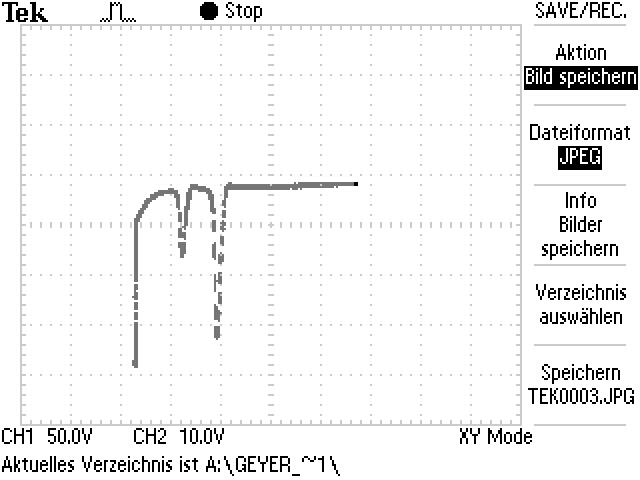
\includegraphics[scale=1]{Auswertung/Daten/TEK0003.jpg}
  \caption{Typisches Signalbild bei einer Resonanzfrequenz von \SI{100}{\kilo\hertz}.}
  \label{abb:signalbild}
\end{figure}
Dabei ist der erste Peak der Grundzustand, in dem die Transmission gegen 0 geht.
Die beiden folgenden Peaks korrespondieren zu $\symup{^{87} Rb}$ bzw. zu $\symup{^{85} Rb}$.
Um das Verhältnis der Amplituden zu bilden, wird das Bild in \textit{GIMP} eingelesen
und die Differenz zwischen der horizontalen Linie und der beiden Peaks gebildet.
Es ergeben sich als \enquote{Tiefen} $T_{1, 2}$ der Peaks
\begin{align}
  T_1 &= \SI{71}{\px} \\
  T_2 &= \SI{153}{\px}
\end{align}
in Pixeln. Damit folgt, dass die Verteilung bei $\sim \SI{32}{\percent}$ ($\symup{^{87} Rb}$)
und $\sim \SI{68}{\percent}$ ($\symup{^{85} Rb}$) liegt. In der Natur liegen die
Isotope in dem Verhältnis $\sim \SI{72}{\percent}$ ($\symup{^{85} Rb}$) und
$\sim \SI{28}{\percent}$ ($\symup{^{87} Rb}$) vor.

\subsection{Abschätzung des quadratischen Zeeman-Effekts}
Zur Abschätzung des quadratischen Zeeman-Effekts wird \eqref{eqn:quadratischer-zeeman}
ausgerechnet. Dabei wird das maximale gemessene magnetische Feld verwendet
(\SI{140.05}{\micro\tesla} für die erste Resonanzstelle und \SI{211.83}{\micro\tesla}
für die zweite). Mit $m_F = 3$ für $\symup{^{85} Rb}$ und $m_F = 2$ für $\symup{^{87} Rb}$
und den entsprechenden Hyperfeinstrukturaufspaltungen aus \cite{anleitung} ergeben sich
\begin{align}
  U_{\symup{HF}_{1}} &= \SI{4.06(6)e-09}{\eV} \\
  U_{\symup{HF}_{2}} &= \SI{4.07(4)e-09}{\eV} \, .
\end{align}

\subsection{Auswertung der Periodendauer}
In \autoref{abb:perioden} sind die gemessenen Periodendauern gegen die RF-Amplitude
aufgetragen. Es wurde ein Fit der Form $f(x) = a + \frac{b}{x-c}$ angefertigt.
Dabei ist zu beachten, dass die beiden ersten Messpunkte beider Messreihen nicht
in den Fit oder den Plot eingeflossen sind, da im Falle der ersten Periode gar keine
Schwingung zu erkennen war und in der zweiten Periode der Wert unter zu großer
Ungenauigkeit aufgenommen wurde.
\FloatBarrier
\begin{figure}
  \centering
  \includegraphics[scale=0.7]{Auswertung/Plots/Perioden.pdf}
  \caption{Periodendauer gegen die RF-Amplitude aufgetragen. Zusätzlich ist ein
  hyperbolischer Fit eingezeichnet.}
  \label{abb:perioden}
\end{figure}
\FloatBarrier
Die Parameter des Fits sind in \autoref{tab:parameter-periode} dargestellt.
\begin{table}
  \centering
  \caption{Parameter des hyperbolischen Fits}
  \label{tab:parameter-periode}
  \begin{tabular}{c c c c}
    \toprule
    Isotop & a / \si{\milli\second} & b / \si{\volt\milli\second} & c / \si{\volt} \\
    \midrule
    $\symup{^{87} Rb}$ & \num{0.03(5)} & \num{1.93(34)} & \num{0.16(21)} \\
    $\symup{^{85} Rb}$ & \num{0.062(19)} & \num{3.09(13)} & \num{0.20(5)} \\
    \bottomrule
  \end{tabular}
\end{table}
Für den Quotienten $b(\symup{^{87} Rb})/b(\symup{^{85} Rb})$ ergibt sich $\num{0.62(11)}$.
In \autoref{sub-abb:87} und \autoref{sub-abb:85} sind die ansteigenden Flanken der
Periodendauern zu sehen.

\begin{figure}
  \centering
  \begin{subfigure}{0.46\textwidth}
    \centering
    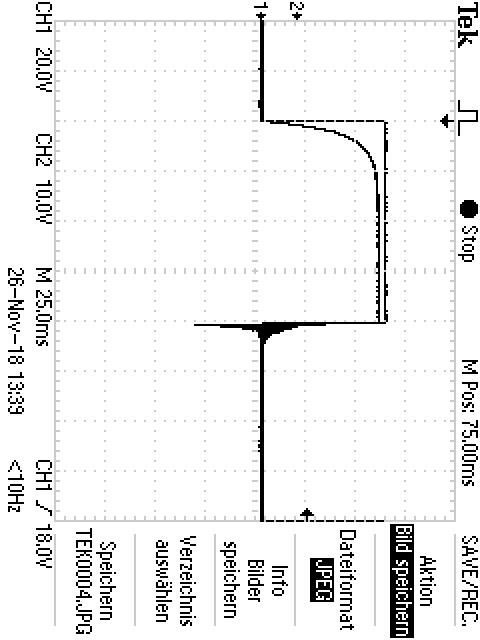
\includegraphics[width=\textwidth]{Auswertung/Daten/TEK0004.jpg}
    \caption{Ansteigende Flanke der Periodendauer für $\symup{^{87} Rb}$.}
    \label{sub-abb:87}
  \end{subfigure}
  \qquad
  \begin{subfigure}{0.46\textwidth}
    \centering
    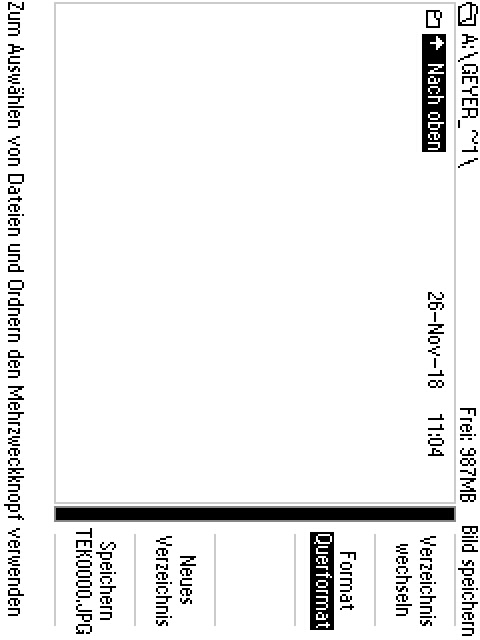
\includegraphics[width=\textwidth]{Auswertung/Daten/TEK0000.jpg}
    \caption{Ansteigende Flanke der Periodendauer für $\symup{^{85} Rb}$.}
    \label{sub-abb:85}
  \end{subfigure}
  \caption{Ansteigende Flanken der Periodendauern für beide Isotope.}
  \label{abb:ansteigende-flanken}
\end{figure}

\section{Diskusion}
